\documentclass[10pt,aspectratio=169]{beamer}
\usetheme[progressbar=frametitle,numbering=fraction,sectionpage=progressbar]{metropolis}
\usepackage[T1]{fontenc}
\usepackage{amsmath,amssymb,mathtools,bm,booktabs,graphicx,xcolor}
\usepackage{tikz}
\usetikzlibrary{arrows.meta,positioning,shapes.geometric,calc,decorations.pathmorphing,decorations.pathreplacing,fit,backgrounds}
\usepackage[most]{tcolorbox}

\definecolor{aBlue}{HTML}{1F77B4}
\definecolor{bRed}{HTML}{D62728}
\definecolor{okGreen}{HTML}{2CA02C}
\definecolor{softGray}{HTML}{F2F2F2}
\setbeamercolor{frametitle}{bg=aBlue!85!black}
\setbeamercolor{progress bar}{fg=bRed}

\newtcolorbox{keybox}[1][Key idea]{colback=aBlue!6,colframe=aBlue,fonttitle=\bfseries\small,title={#1},boxrule=0.6pt,arc=2pt,left=4pt,right=4pt,top=2pt,bottom=2pt}
\newtcolorbox{derivbox}[1][Derivation]{colback=softGray,colframe=black!45,fonttitle=\bfseries\small,title={#1},boxrule=0.5pt,arc=2pt,left=4pt,right=4pt,top=2pt,bottom=2pt}
\newtcolorbox{codebox}[1][In NuWro's code]{colback=okGreen!5,colframe=okGreen!60!black,fonttitle=\bfseries\small,title={#1},boxrule=0.5pt,arc=2pt,left=4pt,right=4pt,top=1pt,bottom=1pt}
\newtcolorbox{warnbox}[1][Careful]{colback=bRed!5,colframe=bRed,fonttitle=\bfseries\small,title={#1},boxrule=0.6pt,arc=2pt,left=4pt,right=4pt,top=2pt,bottom=2pt}

\newcommand{\G}{\Gamma}
\newcommand{\Gh}{\hat\Gamma}
\newcommand{\Ekeff}{E_k^{\rm eff}}
\newcommand{\code}[1]{{\small\texttt{#1}}}
\newcommand{\tagrun}{{\scriptsize\color{okGreen}[run]}}
\newcommand{\tagsrc}[1]{{\scriptsize\color{aBlue}[source: #1]}}
\newcommand{\tagder}{{\scriptsize\color{black!60}[derived]}}

\title{NuWro's intranuclear cascade, and a Sudakov veto version of it}
\subtitle{How the cascade works, what it approximates, how a veto algorithm replaces the time steps,\\ and whether that is worth it}
\author{Josue (Isaacson HEP Theory, MSU) \quad with Claude}
\date{29 October 2026 \quad\textbullet\quad NuWro commit \texttt{f16c937}}

\begin{document}
\maketitle

% =====================================================================
\begin{frame}{Roadmap}
\begin{columns}[T]
\column{0.55\textwidth}
\begin{enumerate}
\item \textbf{The one equation of any cascade}: survival probability $e^{-\int\G}$
\item \textbf{NuWro's cascade (a)}: what it tracks, every factor in its collision rate, what a collision does
\item \textbf{What (a) is approximating}, and the two errors a finite step makes
\item \textbf{The Sudakov veto cascade (b)}: algorithm, proof, how the bound is built
\item \textbf{Validation}: closed forms, (a) at $\Delta\to0$, data, CPU
\item \textbf{Reweighting}: event weights for $\sigma$ and mean-free-path variations
\item \textbf{Verdict}
\end{enumerate}
\column{0.42\textwidth}
\begin{keybox}[Naming used throughout]
\textbf{(a)} = NuWro's cascade as it stands (fixed steps of $\Delta=0.2$ fm).\\[3pt]
\textbf{(b)} = same physics, but the stepping loop replaced by a Sudakov veto algorithm (no steps).
\end{keybox}
\vspace{2pt}
{\small Number tags: \tagrun\ my simulation; \tagsrc{file:line} read in NuWro source; \tagder\ derived on the slide.}
\end{columns}
\end{frame}

% =====================================================================
\section{Part 1 -- The one equation of a cascade}

\begin{frame}{What an intranuclear cascade does}
\begin{columns}[c]
\column{0.5\textwidth}
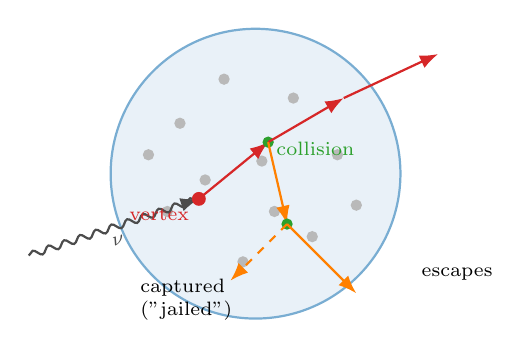
\begin{tikzpicture}[scale=0.8]
  \fill[aBlue!10] (0,0) circle (2.3);
  \draw[aBlue!60,thick] (0,0) circle (2.3);
  \foreach \x/\y in {-1.2/0.8,-0.5/1.5,0.6/1.2,1.3/0.3,0.9/-1.0,-0.2/-1.4,-1.4/-0.6,0.1/0.2,-0.8/-0.1,1.6/-0.5,-1.7/0.3,0.3/-0.6}
     \fill[gray!55] (\x,\y) circle (0.09);
  \draw[decorate,decoration={snake,amplitude=1.2pt,segment length=6pt},thick,black!70,-{Latex}] (-3.6,-1.3) -- (-0.9,-0.4) node[midway,below,sloped]{\scriptsize $\nu$};
  \fill[bRed] (-0.9,-0.4) circle (0.11) node[below left]{\scriptsize vertex};
  \draw[-{Latex},thick,bRed] (-0.9,-0.4) -- (0.2,0.5);
  \fill[okGreen] (0.2,0.5) circle (0.09);
  \draw[-{Latex},thick,bRed] (0.2,0.5) -- (1.4,1.2);
  \draw[-{Latex},thick,orange] (0.2,0.5) -- (0.5,-0.8);
  \fill[okGreen] (0.5,-0.8) circle (0.09);
  \draw[-{Latex},thick,orange] (0.5,-0.8) -- (1.6,-1.9);
  \draw[-{Latex},thick,orange,dashed] (0.5,-0.8) -- (-0.4,-1.7);
  \draw[-{Latex},thick,bRed] (1.4,1.2) -- (2.9,1.9);
  \node[font=\scriptsize,align=left] at (3.2,-1.6) {escapes};
  \node[font=\scriptsize,align=left] at (-1.1,-2.0) {captured\\("jailed")};
  \node[font=\scriptsize,okGreen] at (0.95,0.4) {collision};
\end{tikzpicture}
\column{0.48\textwidth}
\small
\begin{itemize}
\item The neutrino interacts with one nucleon (the \emph{vertex}).
\item The outgoing hadrons must leave a nucleus full of other nucleons.
\item On the way they can \textbf{rescatter}, knock out nucleons, make or absorb pions, or be captured.
\item A \textbf{cascade} treats this classically: straight lines between collisions, collisions at random points.
\end{itemize}
\begin{keybox}
The transport only has to answer: \textbf{where along its straight line does a hadron collide next?}
\end{keybox}
\end{columns}
\end{frame}

\begin{frame}{The survival probability}
\small
\begin{columns}[T]
\column{0.52\textwidth}
Let $\G(\ell)$ be the collision rate per unit length (\emph{hazard}) at path length $\ell$:
\[
\G(\ell)=\rho(\mathbf r(\ell))\,\sigma \qquad[\text{fm}^{-1}]
\]
\begin{derivbox}
$S(\ell)=$ probability of no collision in $[0,\ell]$.\\
To survive to $\ell+d\ell$: survive to $\ell$, then not collide in $d\ell$:
$S(\ell+d\ell)=S(\ell)\,\big(1-\G(\ell)\,d\ell\big)\ \Rightarrow\ \dfrac{dS}{d\ell}=-\G(\ell)\,S(\ell)$
\[
\boxed{S(\ell)=\exp\Big[-\int_0^\ell\G(\ell')\,d\ell'\Big]}
\]
First collision at $\ell$: \ $p(\ell)=-\dfrac{dS}{d\ell}=\G(\ell)\,e^{-\int_0^\ell\G}$.
\end{derivbox}
\column{0.45\textwidth}
\footnotesize
\begin{keybox}[Numbers to keep in mind]
$\rho_0=0.16$ fm$^{-3}$, $\sigma_{NN}=40$ mb $=4$ fm$^2$\\
$\Rightarrow\ \G=0.64$ fm$^{-1}$, mean free path $\lambda=1/\G\approx1.6$ fm.\\[2pt]
A $^{12}$C diameter is $\approx5$ fm: a few mean free paths.
\end{keybox}
In parton showers $S$ is the \textbf{Sudakov factor} (no emission between two scales).
\begin{warnbox}[The difficulty]
$\G$ varies along the path (density, energy, correlations, target motion): $\int\G$ has no closed form, so $S$ cannot be inverted directly.
\end{warnbox}
\end{columns}
\end{frame}

\begin{frame}{When $\G$ is constant, sampling is trivial}
\centering
\includegraphics[width=0.66\textwidth]{figs/survival.pdf}
\begin{columns}[T]
\column{0.5\textwidth}
\begin{derivbox}[Inverse-transform sampling]
CDF $F(\ell)=1-e^{-\G\ell}$. With $u\sim U(0,1)$, set $F(\lambda)=u$:
\[
\lambda=-\frac{\ln(1-u)}{\G}\quad(\text{same law as }-\ln u/\G).
\]
\end{derivbox}
\column{0.47\textwidth}
\begin{keybox}[Two ways out when $\G$ varies]
\textbf{(a) step it:} pretend $\G$ is constant over short steps $\Delta$.\\
\textbf{(b) veto it:} sample with a constant \emph{upper bound} $\Gh\ge\G$, then correct.
\end{keybox}
\end{columns}
\end{frame}

\begin{frame}{The two strategies, side by side}
\centering
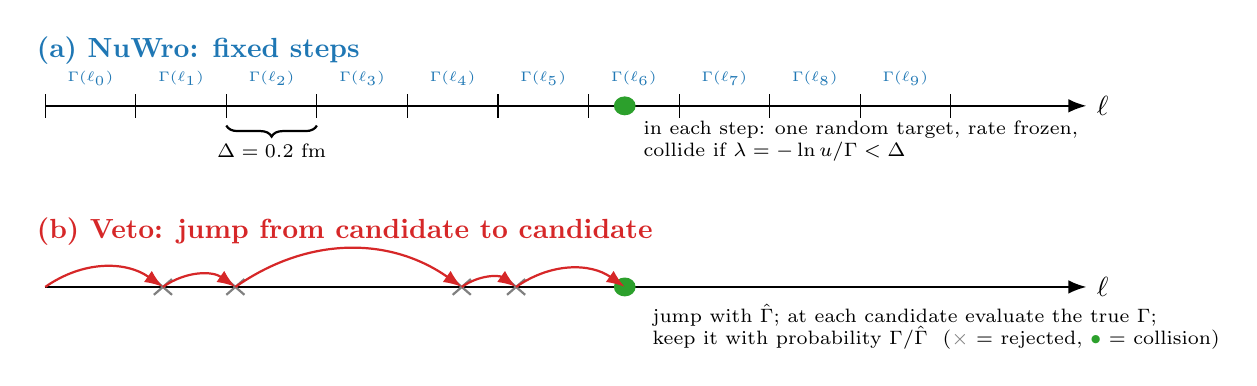
\begin{tikzpicture}[x=1.15cm,y=1cm]
  % (a)
  \node[anchor=west,font=\bfseries,aBlue] at (-0.2,2.9) {(a) NuWro: fixed steps};
  \draw[thick,-{Latex}] (0,2.2) -- (11.5,2.2) node[right]{$\ell$};
  \foreach \i in {0,...,10} {\draw (\i,2.05) -- (\i,2.35);}
  \foreach \i in {0,...,9} {\node[font=\tiny,aBlue] at (\i+0.5,2.55) {$\G(\ell_\i)$};}
  \draw[decorate,decoration={brace,amplitude=4pt},thick] (3,1.95) -- (2,1.95) node[midway,below=3pt,font=\scriptsize]{$\Delta=0.2$ fm};
  \fill[okGreen] (6.4,2.2) circle (0.12); \node[font=\scriptsize,okGreen,above] at (6.4,2.3) {};
  \node[font=\scriptsize,align=left,anchor=west] at (6.5,1.75) {in each step: one random target, rate frozen,\\ collide if $\lambda=-\ln u/\G<\Delta$};
  % (b)
  \node[anchor=west,font=\bfseries,bRed] at (-0.2,0.6) {(b) Veto: jump from candidate to candidate};
  \draw[thick,-{Latex}] (0,-0.1) -- (11.5,-0.1) node[right]{$\ell$};
  \foreach \x/\a in {1.3/0,2.1/0,4.6/0,5.2/0,6.4/1} {
     \ifnum\a=1 \fill[okGreen] (\x,-0.1) circle (0.12); \else \draw[thick,gray] (\x-0.1,-0.2)--(\x+0.1,0.0) (\x-0.1,0.0)--(\x+0.1,-0.2); \fi}
  \draw[-{Latex},bRed,thick] (0,-0.1) to[bend left=35] (1.3,-0.1);
  \draw[-{Latex},bRed,thick] (1.3,-0.1) to[bend left=35] (2.1,-0.1);
  \draw[-{Latex},bRed,thick] (2.1,-0.1) to[bend left=35] (4.6,-0.1);
  \draw[-{Latex},bRed,thick] (4.6,-0.1) to[bend left=35] (5.2,-0.1);
  \draw[-{Latex},bRed,thick] (5.2,-0.1) to[bend left=35] (6.4,-0.1);
  \node[font=\scriptsize,align=left,anchor=west] at (6.6,-0.6) {jump with $\Gh$; at each candidate evaluate the true $\G$;\\ keep it with probability $\G/\Gh$ \ (\textcolor{gray}{$\times$} = rejected, \textcolor{okGreen}{$\bullet$} = collision)};
\end{tikzpicture}
\vspace{6pt}
\begin{keybox}
(a)'s accuracy depends on $\Delta$ (an approximation to $e^{-\int\G}$). (b) is exact for \emph{any} valid bound $\Gh$; the bound only affects speed.
\end{keybox}
\end{frame}

% =====================================================================
\section{Part 2 -- NuWro's cascade (a)}

\begin{frame}{What NuWro keeps track of}
\begin{columns}[T]
\column{0.55\textwidth}
\begin{tabular}{@{}ll@{}}
\toprule
\multicolumn{2}{@{}l}{\textbf{each particle in flight}} \\
\midrule
$\mathbf r,\ t$ & position and a time coordinate\\
$\mathbf p$ & momentum\\
\code{his\_fermi} & its potential (Fermi energy) \\
\code{travelled} $=s$ & distance since created / last scattered\\
\midrule
\multicolumn{2}{@{}l}{\textbf{the residual nucleus}}\\
\midrule
$Z_r,\ N_r$ & protons, neutrons still inside\\
\midrule
\multicolumn{2}{@{}l}{\textbf{the event}}\\
\midrule
\code{parts} & FIFO queue of particles to move\\
\code{nod[]} & counters of collisions by type\\
\bottomrule
\end{tabular}
\column{0.42\textwidth}
\begin{codebox}
\code{particle.h:286}: \code{krok(dl)} moves $\mathbf r\mathrel{+}=dl\,\hat{\mathbf v}$, $t\mathrel{+}=dl/v$, \code{travelled}$\mathrel{+}=dl$\\[2pt]
\code{kaskada7.h:54}: \code{queue<particle> parts}\\[2pt]
\code{nucleus.h:119}: \code{Zr(), Nr(), Ar()}
\end{codebox}
\vspace{2pt}
\begin{keybox}[Why $s$ matters]
The correlation factor (later) depends on how far the particle has gone since its last collision. So $s$ must be part of the state.
\end{keybox}
\end{columns}
\end{frame}

\begin{frame}{The main loop of (a)}
\centering
\resizebox{\textwidth}{!}{%
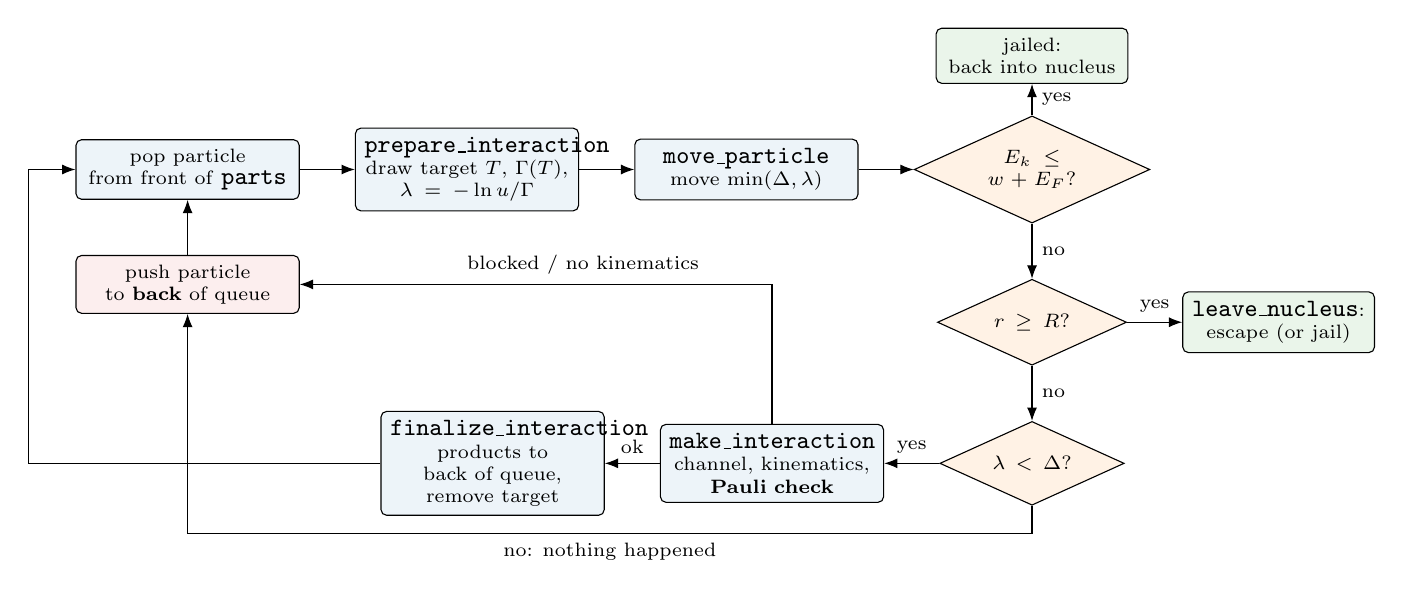
\begin{tikzpicture}[node distance=4mm and 7mm, every node/.style={font=\scriptsize},
  box/.style={draw,rounded corners=2pt,fill=aBlue!8,align=center,minimum height=7mm,text width=26mm},
  dec/.style={draw,diamond,aspect=2.2,fill=orange!10,align=center,inner sep=1pt,text width=17mm},
  outb/.style={draw,rounded corners=2pt,fill=okGreen!10,align=center,minimum height=7mm,text width=22mm},
  >={Latex}]
\node[box] (pop) {pop particle\\from front of \code{parts}};
\node[box,right=of pop] (prep) {\code{prepare\_interaction}\\ draw target $T$, $\G(T)$,\\ $\lambda=-\ln u/\G$};
\node[box,right=of prep] (move) {\code{move\_particle}\\ move $\min(\Delta,\lambda)$};
\node[dec,right=of move] (jail) {$E_k\le w+E_F$?};
\node[outb,above=of jail] (jailed) {jailed:\\ back into nucleus};
\node[dec,below=7mm of jail] (outside) {$r\ge R$?};
\node[outb,right=of outside] (esc) {\code{leave\_nucleus}:\\ escape (or jail)};
\node[dec,below=7mm of outside] (coll) {$\lambda<\Delta$?};
\node[box,left=of coll] (make) {\code{make\_interaction}\\ channel, kinematics,\\ \textbf{Pauli check}};
\node[box,left=of make] (fin) {\code{finalize\_interaction}\\ products to back of queue,\\ remove target};
\node[box,below=7mm of pop,fill=bRed!8] (push) {push particle\\ to \textbf{back} of queue};
\draw[->] (pop)--(prep); \draw[->] (prep)--(move); \draw[->] (move)--(jail);
\draw[->] (jail)--node[right]{yes}(jailed); \draw[->] (jail)--node[right]{no}(outside);
\draw[->] (outside)--node[above]{yes}(esc); \draw[->] (outside)--node[right]{no}(coll);
\draw[->] (coll)--node[above]{yes}(make);
\draw[->] (make)--node[above]{ok}(fin);
\draw[->] (coll.south) |- ++(0,-0.35) -| node[pos=0.25,below]{no: nothing happened} (push.south);
\draw[->] (make.north) |- node[pos=0.7,above]{blocked / no kinematics} (push.east);
\draw[->] (push)--(pop);
\draw[->] (fin.west) -| ($(push.south west)+(-0.6,0)$) |- (pop.west);
\end{tikzpicture}}
\vspace{2pt}
{\scriptsize \tagsrc{kaskada7.cc:72--93 (loop), 681--763 (prepare), 766--819 (move), 823--864 (leave), 867--1024 (make), 1027--1144 (finalize)}}
\end{frame}

\begin{frame}{One step of (a), in equations}
\begin{columns}[T]
\column{0.55\textwidth}
At the start of each step, at position $r$, NuWro computes
\[
\G \;=\; \rho_n(r)\,\sigma_n \;+\; \rho_p(r)\,\sigma_p ,
\]
where $\sigma_{n,p}$ is the cross section on a neutron/proton target, evaluated for \textbf{one randomly drawn target nucleon $T$}.\\[4pt]
Then
\[
\lambda=-\frac{\ln u}{\G},\qquad
\text{move by }\min(\Delta,\lambda),
\]
\[
\text{collide iff }\lambda<\Delta \ \ (\text{and still inside}).
\]
Isospin of the target: proton with probability $\rho_p\sigma_p/\G$.
\column{0.42\textwidth}
\begin{codebox}
{\scriptsize\texttt{:747 xsec = dens\_n*xsec\_n + dens\_p*xsec\_p}\\
\texttt{:753 freepath = -log(frandom())/xsec}\\
\texttt{:768 p->krok(min(max\_step, freepath))}}
\end{codebox}
\begin{keybox}[What this is]
The exact constant-rate sampler, with $\G$ \emph{frozen at the start of the step} and computed from \emph{one} target. No collision in $\Delta$ $\Rightarrow$ start over with a new rate and a new target.\\[2pt]
\textbf{Default} $\Delta=0.2$ fm (\code{step}, \code{params\_all.h:135}).
\end{keybox}
\end{columns}
\end{frame}

\begin{frame}{Ingredient 1: the nucleus}
\centering
\includegraphics[width=0.88\textwidth]{figs/density.pdf}
\begin{columns}[T]
\column{0.5\textwidth}
\small
\begin{itemize}
\item $\rho(r)=\rho_{\rm FB}(r)\,A_r/A$: experimental point density, rescaled as nucleons are removed. \tagsrc{nucleus.cc:69}
\item $\rho_n=\rho\,N_r/A_r$, \ $\rho_p=\rho\,Z_r/A_r$. \tagsrc{kaskada7.cc:714}
\end{itemize}
\column{0.47\textwidth}
\small
\begin{itemize}
\item Local Fermi gas: $k_F(r)=(3\pi^2\rho_{p,n}(r))^{1/3}$, $E_F=\sqrt{k_F^2+M^2}-M$. \tagsrc{nucleus.h:181}
\item A particle "leaves" at $r\ge R=8.0$ fm. \tagrun
\end{itemize}
\end{columns}
\end{frame}

\begin{frame}{Ingredient 2: the target nucleon and $\Ekeff$}
\begin{columns}[T]
\column{0.42\textwidth}
\centering
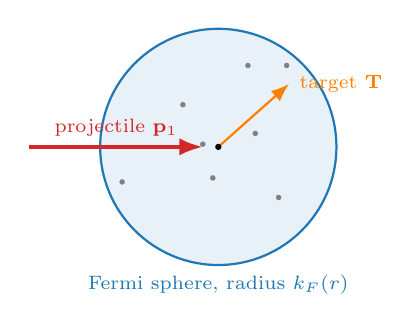
\begin{tikzpicture}[scale=1.0]
  \fill[aBlue!10] (0,0) circle (1.5);
  \draw[aBlue,thick] (0,0) circle (1.5);
  \node[aBlue,font=\scriptsize] at (0,-1.75) {Fermi sphere, radius $k_F(r)$};
  \draw[-{Latex},thick,orange] (0,0) -- (0.9,0.8) node[right,font=\scriptsize]{target $\mathbf T$};
  \fill (0,0) circle (0.04);
  \draw[-{Latex},very thick,bRed] (-2.4,0) -- (-0.2,0) node[midway,above,font=\scriptsize]{projectile $\mathbf p_1$};
  \foreach \a/\r in {20/0.5,70/1.1,130/0.7,200/1.3,260/0.4,320/1.0,170/0.2,50/1.35}
     \fill[gray] (\a:\r) circle (0.035);
\end{tikzpicture}
\column{0.56\textwidth}
\begin{itemize}
\item NuWro draws $\mathbf T$ \textbf{uniformly inside the local Fermi sphere}. \tagsrc{nucleus.cc:138}
\item The cross section is evaluated at the projectile's kinetic energy \textbf{in the target rest frame}:
\end{itemize}
\begin{derivbox}[$\Ekeff$ from an invariant]
$E_1'=\dfrac{p_1\cdot T}{m_2}=\dfrac{E_1E_2-\mathbf p_1\!\cdot\!\mathbf T}{m_2}$,\qquad $\Ekeff=E_1'-m_1$.\\[3pt]
Range over the sphere ($|\mathbf T|\le k_F$):
\[
\Ekeff\in\Big[\tfrac{E_1E_2-p_1k_F}{m_2}-m_1,\ \tfrac{E_1E_2+p_1k_F}{m_2}-m_1\Big],
\]
and $\Ekeff=0$ is possible if a target can move \emph{with} the projectile ($p_1 m_2/m_1\le k_F$).
\end{derivbox}
\end{columns}
\end{frame}

\begin{frame}{Ingredient 3: the free NN cross section}
\centering
\includegraphics[width=0.88\textwidth]{figs/nnxs.pdf}\\
\begin{columns}[T]
\column{0.5\textwidth}\small
$\sigma_{np}$ at $\Ekeff\to0$ is $\sim13$ b (the $np$ singlet). This matters twice later: for the step error of (a) and the efficiency of (b).
\column{0.47\textwidth}\small
After a collision is decided, $f_{\rm inel}$ picks elastic / single-$\pi$ / double-$\pi$. It is \emph{not} a separate hazard. \tagsrc{Interaction.cc:690--700}
\end{columns}
\end{frame}

\begin{frame}{The same projectile sees very different $\sigma$ from different targets}
\centering
\includegraphics[width=0.98\textwidth]{figs/sigma_spread.pdf}
\begin{keybox}
For a fast projectile (800 MeV) every target gives about the same $\sigma$. For a slow one (40 MeV) $\sigma$ ranges over two orders of magnitude depending on which target was drawn.
\textbf{This spread is the root of (a)'s step error and of (b)'s low acceptance.} \hfill{\scriptsize nuclear centre, $k_F=263$ MeV; NuWro table}
\end{keybox}
\end{frame}

\begin{frame}{Ingredient 4: in-medium modifications}
\begin{columns}[T]
\column{0.55\textwidth}
\textbf{Elastic part}: Pandharipande--Pieper \tagsrc{Interaction.cc:337--357}
\[
\mathrm{mod}=\frac{|\mathbf k_1-\mathbf k_2|/M}{\big|\mathbf k_1/m_1^*-\mathbf k_2/m_2^*\big|}\;\frac{m_3^*}{M}
\]
\[
m^*(k)=\frac{M}{1+a\,/\,(1+k^2/\lambda^2)^2},\quad a=\frac{2M|\beta|}{\lambda^2}
\]
with $\beta=-116\,\rho/\rho_0$ MeV, $\lambda=(3.29-0.373\,\rho/\rho_0)$ fm$^{-1}$.\\[4pt]
\textbf{Inelastic part}: $\ \times(1-0.2\,\rho/\rho_0)$. \tagsrc{Interaction.cc:361}\\[4pt]
Combined: $\sigma=\sigma_{\rm free}\big[(1-f_{\rm inel})\,\mathrm{mod}+f_{\rm inel}(1-0.2\rho/\rho_0)\big]$.
\column{0.42\textwidth}
\begin{keybox}["Effective Pauli" factor]
If the projectile has $E_k<40$ MeV, the \emph{unlike-pair} ($np$) cross section is multiplied by $0.9$. \tagsrc{Interaction.cc:380--389}
\end{keybox}
\begin{keybox}[Meaning]
Nucleons in medium have a smaller effective mass, which reduces the flux and hence $\sigma$. The factor depends on the density \emph{and} on both momenta, so again on the random target.
\end{keybox}
\end{columns}
\end{frame}

\begin{frame}{Ingredient 5: short-range correlations and the mfp scale}
\centering
\includegraphics[width=0.74\textwidth]{figs/corr.pdf}
\[
\sigma_c\;\to\;\sigma_c\;\frac{\mathrm{corr}_c(s)}{\mathrm{norm}_c(r)}\;\frac{1}{s_{\rm mfp}},\qquad s_{\rm mfp}=\texttt{kaskada\_NN\_mfp\_scale}=0.76
\]
\vspace{-4pt}
\begin{columns}[T]
\column{0.5\textwidth}\small
Just after a collision ($s\to0$) the neighbours are depleted: the "correlation hole". Tables from ANL ab-initio densities. \tagsrc{kaskada7.cc:720--745}
\column{0.47\textwidth}\small
\textbf{Switched off} for a beam nucleon before its first collision in \code{beam\_placement=2} (the $\sigma_R$ mode). \tagsrc{kaskada7.cc:727}
\end{columns}
\end{frame}

\begin{frame}{Putting it together: the hazard NuWro is computing}
\begin{tcolorbox}[colback=aBlue!5,colframe=aBlue,boxrule=0.8pt]
\begin{align*}
\G_c(\ell)\;=\;&\mathbb E_T\!\Big[\rho_c(r)\;\sigma_{{\rm free},c}\big(\Ekeff(\mathbf p_1,T)\big)\,
\big[(1\!-\!f_{\rm inel})\,\mathrm{mod}(\rho,\mathbf p_1,T)+f_{\rm inel}(1\!-\!0.2\tfrac{\rho}{\rho_0})\big]\Big]\\
&\times\;0.9^{[E_k<40,\,np]}\;\;
\frac{\mathrm{corr}_c(s)}{\mathrm{norm}_c(r)}\;\;\frac{1}{s_{\rm mfp}}
\end{align*}
\end{tcolorbox}
\begin{columns}[T]
\column{0.5\textwidth}
\begin{itemize}\small
\item $c\in\{n,p\}$: the \textbf{isospin of the target} is the channel.
\item $r=|\mathbf r(\ell)|$, $s=s_0+\ell$: position and distance since last collision.
\item $\mathbb E_T$: average over targets in the local Fermi sphere.
\item Pions: $\sigma$ from tables in $(E_k,\rho)$, no target dependence. \tagsrc{Interaction.cc:403--424}
\end{itemize}
\column{0.47\textwidth}
\begin{warnbox}[Two things (a) does not do]
(1) It never averages over $T$: each step uses \emph{one} $T$.\\
(2) It never integrates $\G$ along the path: each step uses $\G$ at the step's start.\\[2pt]
Both become exact only as $\Delta\to0$.
\end{warnbox}
\end{columns}
\end{frame}

\begin{frame}{What a collision does}
\small
\begin{columns}[T]
\column{0.55\textwidth}
\begin{enumerate}
\item \textbf{Target isospin:} proton with $\rho_p\sigma_p/\G$.
\item \textbf{Process} from the \emph{free} inelastic fraction at $\Ekeff$: elastic $(1-f_{\rm inel})$, else $1\pi$ or $2\pi$ (falls back if below threshold).
\item \textbf{Orientation:} flip $\mathbf T\to-\mathbf T$ with probability $\propto\sigma(E_{k2})$ vs $\sigma(E_{k1})$. \tagsrc{Interaction.cc:668--687}
\item \textbf{Kinematics}, retried up to 100 times. \tagsrc{kaskada7.cc:975--989}
\item \textbf{Pauli check} on every outgoing nucleon (next slide).
\item \textbf{Bookkeeping}: products at the same point with $s=0$, to the back of the queue; target removed. \tagsrc{kaskada7.cc:1081--1141}
\end{enumerate}
\column{0.42\textwidth}
\begin{keybox}[The nucleus changes]
After every successful collision $Z_r,N_r$ change, so the density and $k_F$ seen by \emph{every} other particle change too. A fully correct algorithm must take that into account in time order.
\end{keybox}
\end{columns}
\end{frame}

\begin{frame}{Pauli blocking: a collision that does not happen}
\small
\begin{columns}[c]
\column{0.42\textwidth}
\centering
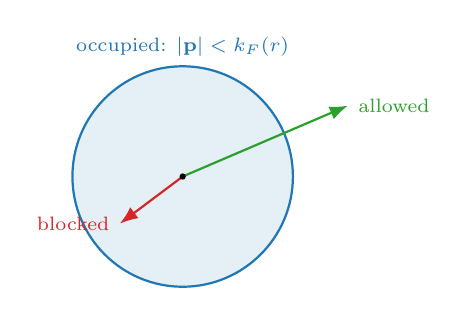
\begin{tikzpicture}[scale=1.0]
  \fill[aBlue!12] (0,0) circle (1.4); \draw[aBlue,thick] (0,0) circle (1.4);
  \node[aBlue,font=\scriptsize] at (0,1.65) {occupied: $|\mathbf p|<k_F(r)$};
  \draw[-{Latex},thick,okGreen] (0,0) -- (2.1,0.9) node[right,font=\scriptsize,align=left]{allowed};
  \draw[-{Latex},thick,bRed] (0,0) -- (-0.8,-0.6) node[left,font=\scriptsize,align=right]{blocked};
  \fill (0,0) circle(0.04);
\end{tikzpicture}
\column{0.56\textwidth}
\begin{itemize}
\item Any outgoing nucleon with $|\mathbf p|<k_F^{\rm loc}(r)$ $\Rightarrow$ the collision is \textbf{blocked}. \tagsrc{kaskada7.cc:1001, nucleus.h:234}
\item NuWro then simply \textbf{discards the collision}: the particle continues from the collision point with the same momentum and $s$. \tagsrc{kaskada7.cc:84--90}
\end{itemize}
\begin{derivbox}[In continuous time this is "thinning"]
If a collision passes the Pauli check with probability $q$, real collisions happen at rate $\G_{\rm eff}=q\,\G$.\\
(b) keeps this exactly: an accepted candidate that is then blocked is discarded, and the particle goes on.
\end{derivbox}
\end{columns}
\end{frame}

\begin{frame}{Leaving the nucleus, and being captured ("jailing")}
\small
\begin{columns}[T]
\column{0.5\textwidth}
\centering
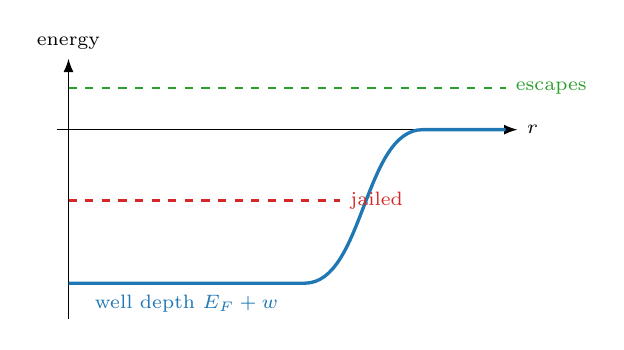
\begin{tikzpicture}[x=0.75cm,y=0.75cm]
  \draw[-{Latex}] (-0.2,0) -- (7.6,0) node[right,font=\scriptsize]{$r$};
  \draw[-{Latex}] (0,-3.2) -- (0,1.2) node[above,font=\scriptsize]{energy};
  \draw[very thick,aBlue] (0,-2.6) -- (4,-2.6) .. controls (5,-2.6) and (5,0) .. (6,0) -- (7.4,0);
  \node[aBlue,font=\scriptsize] at (2,-2.95) {well depth $E_F+w$};
  \draw[dashed,okGreen,thick] (0,0.7) -- (7.4,0.7) node[right,font=\scriptsize]{escapes};
  \draw[dashed,bRed,thick] (0,-1.2) -- (4.6,-1.2) node[right,font=\scriptsize]{jailed};
\end{tikzpicture}
\\{\scriptsize $w=7$ MeV ("work function", \code{kaskada\_w})}
\column{0.48\textwidth}
\begin{itemize}\small
\item A nucleon with $E_k\le w+E_F$ is \textbf{jailed}: put back into the nucleus. Checked after every step, at the surface, and for every product. \tagsrc{kaskada7.cc:795, 831, 1089}
\item On escape, its energy is reduced by $E_F+w$. \tagsrc{kaskada7.cc:839}
\end{itemize}
\begin{derivbox}[Jailing never happens mid-flight]
Let $J=E_k-\texttt{his\_fermi}$. Outside the SF branch neither term changes along a path. Inside it, NuWro adds $E_F(r)-E_F(r_0)$ to $E_k$ and sets \code{his\_fermi}$=E_F(r)$ (\code{kaskada7.cc:775--783}). So $J$ is constant on a straight path, and the test $J\le w$ can only change at creation or at the surface. \tagder
\end{derivbox}
\end{columns}
\end{frame}

\begin{frame}{Who moves first? Rounds versus time}
\centering
\resizebox{\textwidth}{!}{%
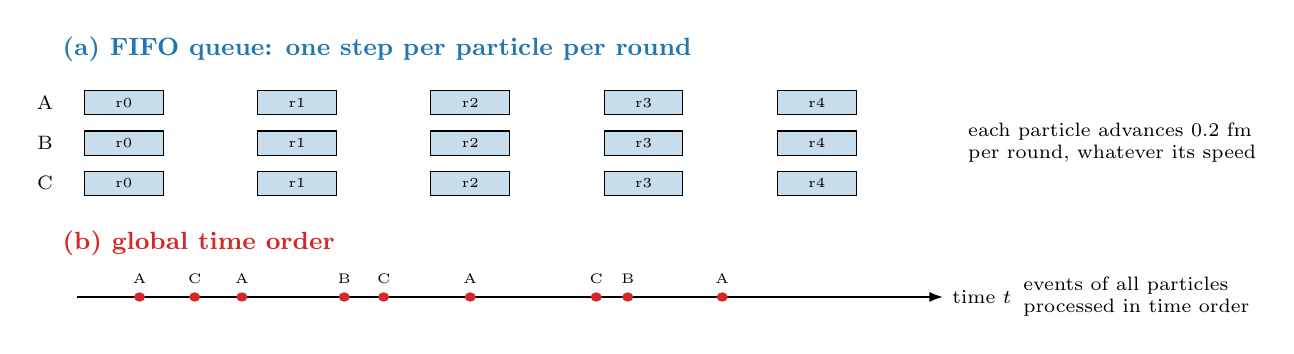
\begin{tikzpicture}[x=1cm,y=0.85cm]
  \node[anchor=west,font=\bfseries\small,aBlue] at (-0.3,3.5) {(a) FIFO queue: one step per particle per round};
  \foreach \p/\y/\v in {A/2.7/1.0,B/2.1/0.45,C/1.5/0.75} {
     \node[font=\scriptsize] at (-0.4,\y) {\p};
     \foreach \k in {0,...,4} { \draw[fill=aBlue!25] (\k*2.2+0.1,\y-0.18) rectangle ++(1.0,0.36); \node[font=\tiny] at (\k*2.2+0.6,\y) {r\k};}
  }
  \node[font=\scriptsize,align=left,anchor=west] at (11.2,2.1) {each particle advances 0.2 fm\\per round, whatever its speed};
  \node[anchor=west,font=\bfseries\small,bRed] at (-0.3,0.6) {(b) global time order};
  \draw[-{Latex}] (0,-0.2) -- (11,-0.2) node[right,font=\scriptsize]{time $t$};
  \foreach \x/\l in {0.8/A,1.5/C,2.1/A,3.4/B,3.9/C,5.0/A,6.6/C,7.0/B,8.2/A} {\fill[bRed] (\x,-0.2) circle(0.07); \node[font=\tiny,above] at (\x,-0.15) {\l};}
  \node[font=\scriptsize,align=left,anchor=west] at (11.9,-0.2) {events of all particles\\ processed in time order};
\end{tikzpicture}}
\vspace{4pt}
\begin{keybox}
The order only matters through changes of the nucleus ($Z_r,N_r$) caused by other particles' collisions: a $\sim1/A$ effect per collision. It cannot change $\sigma_R$ or the transparency, which depend only on the first collision of the leading nucleon.
\end{keybox}
\end{frame}

\begin{frame}{How NuWro measures $\sigma_R$ and transparency}
\begin{columns}[c]
\column{0.5\textwidth}
\centering
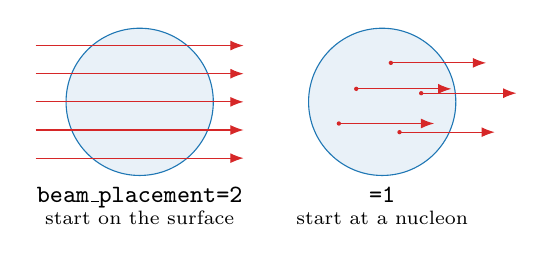
\begin{tikzpicture}[scale=0.55]
  \fill[aBlue!10] (0,0) circle (1.7); \draw[aBlue] (0,0) circle (1.7);
  \foreach \y in {-1.3,-0.65,0,0.65,1.3} \draw[-{Latex},bRed] (-2.4,\y) -- (2.4,\y);
  \node[font=\scriptsize,align=center] at (0,-2.4) {\code{beam\_placement=2}\\start on the surface};
  \begin{scope}[xshift=5.6cm]
  \fill[aBlue!10] (0,0) circle (1.7); \draw[aBlue] (0,0) circle (1.7);
  \foreach \x/\y in {-0.6/0.3,0.4/-0.7,0.2/0.9,-1.0/-0.5,0.9/0.2}{ \fill[bRed] (\x,\y) circle(0.05); \draw[-{Latex},bRed] (\x,\y) -- ++(2.2,0); }
  \node[font=\scriptsize,align=center] at (0,-2.4) {\code{=1}\\start at a nucleon};
  \end{scope}
\end{tikzpicture}
\column{0.48\textwidth}
\[
\sigma_R=\pi(0.999R)^2\;P(\ge1\text{ real collision})
\]
\[
T=P(0\text{ real collisions}),\quad \text{plotted vs }Q^2\simeq2M T_p
\]
as in NuWro's own validation code. \tagsrc{calculations.cc:1588, nucleusmaker.h:29--41}\\[4pt]
\begin{keybox}
Both observables only ask "did the leading nucleon collide at least once?". Later collisions of secondaries do not enter.
\end{keybox}
\end{columns}
\end{frame}

\begin{frame}{Four things I found in (a) along the way}
\begin{enumerate}
\item \textbf{Uninitialised event flags in \code{kaskada} (beam mode).} \code{event::flag} is never set (\code{event1.h:10--27, 91}). In my build \code{flag.qel} was non-zero in 100\% of events \tagrun, so every nucleon runs the QE spectral-function code path: the consistent-target rate, the potential-well energy updates, and $+E_F+w$ on entry. This is undefined behaviour; it may differ between builds.
\item \textbf{Pauli-blocked pion absorption still removes nucleons.} \code{pion\_abs} changes $Z_r,N_r$ \emph{before} the Pauli check and does not undo it. \tagsrc{Interaction.h:574--680}
\item \textbf{A failed \code{remove\_nucleon} duplicates particles}: products are already queued (\code{kaskada7.cc:1110}), then the projectile is queued again (\code{:89}).
\item \textbf{The cascade ignores the \code{pauli\_blocking} parameter.} \tagsrc{kaskada7.cc:1001}
\end{enumerate}
\begin{keybox}
(b) reproduces whatever (a) does in all four cases. These are reports for the NuWro developers, independent of the veto algorithm.
\end{keybox}
\end{frame}

% =====================================================================
\section{Part 3 -- What (a) approximates, and its two errors}

\begin{frame}{The continuous-time process behind (a)}
\small
\begin{tcolorbox}[colback=aBlue!5,colframe=aBlue,boxrule=0.8pt,title=Target process,fonttitle=\bfseries\small]
Each particle moves on a straight line. In channel $c\in\{n,p\}$ it collides with hazard $\G_c(\ell)$ of slide ``Putting it together'' (the \textbf{average} over targets), with target law $\propto\G_c(T)\,f(T)$. Pauli blocking thins the collisions. All particles are advanced in \textbf{global time}; the nucleus changes after each collision.
\end{tcolorbox}
\begin{columns}[T]
\column{0.5\textwidth}
\begin{derivbox}[It is Markov]
Every hazard depends only on the current state $\{(\mathbf r,t,\mathbf p,\texttt{his\_fermi},s)_i,\ Z_r,N_r\}$; targets are drawn fresh at every evaluation. Without $s$ in the state the SRC factor would make it non-Markov. \tagder
\end{derivbox}
\column{0.47\textwidth}
\begin{derivbox}[(a) converges to it as $\Delta\to0$]
One step: $P(\text{coll})=\mathbb E_T\big[1-e^{-\G(T)\Delta}\big]=\langle\G\rangle\Delta+O(\Delta^2)$.\\
The struck target is drawn with weight $\G(T)\Delta$, i.e.\ law $\propto\G(T)f(T)$.\\
So: hazard $\to\langle\G\rangle_T$, target law $\to\G f/\langle\G\rangle$. \tagder
\end{derivbox}
\end{columns}
\end{frame}

\begin{frame}{Error 1 of a finite step: the frozen rate}
\begin{columns}[c]
\column{0.5\textwidth}
\centering
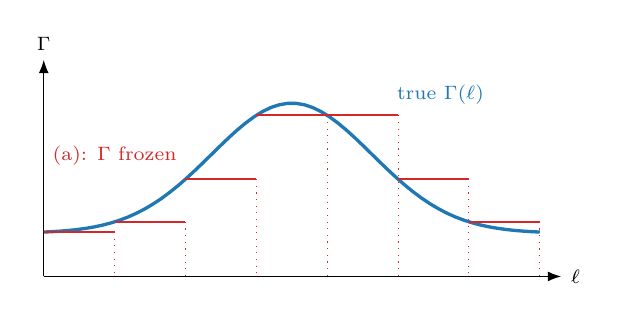
\begin{tikzpicture}[x=0.9cm,y=2.2cm]
  \draw[-{Latex}] (0,0) -- (7.3,0) node[right,font=\scriptsize]{$\ell$};
  \draw[-{Latex}] (0,0) -- (0,1.25) node[above,font=\scriptsize]{$\G$};
  \draw[very thick,aBlue,domain=0:7,samples=60] plot (\x,{0.25+0.75*exp(-((\x-3.5)/1.6)^2)});
  \foreach \i in {0,...,6} {
     \pgfmathsetmacro{\g}{0.25+0.75*exp(-((\i-3.5)/1.6)^2)}
     \draw[thick,bRed] (\i,\g) -- (\i+1,\g);
     \draw[bRed,dotted] (\i+1,\g) -- (\i+1,0);
  }
  \node[aBlue,font=\scriptsize] at (5.6,1.05) {true $\G(\ell)$};
  \node[bRed,font=\scriptsize] at (1.0,0.7) {(a): $\G$ frozen};
\end{tikzpicture}
\column{0.48\textwidth}
Inside a step (a) uses $\G(\ell_0)$ at the start. The correct survival over the step is
\[
e^{-\int_{\ell_0}^{\ell_0+\Delta}\G}=e^{-\G(\ell_0)\Delta-\frac12\G'(\ell_0)\Delta^2+\dots}
\]
so the error per step is $O(\G'\Delta^2)$, i.e.\ $O(\Delta)$ over the whole path. \tagder\\[4pt]
\begin{keybox}
This error is small for NuWro: density changes on a scale of $\sim$1 fm, and the step is 0.2 fm.
\end{keybox}
\end{columns}
\end{frame}

\begin{frame}{Error 2 of a finite step: one random target (Jensen)}
\small
\begin{columns}[T]
\column{0.5\textwidth}
\begin{derivbox}[Effective rate of (a) over one step]
(a) survives a step with probability $\mathbb E_T\big[e^{-\G(T)\Delta}\big]$. Its effective rate is
\[
\begin{aligned}
\G_{\rm eff}&=-\tfrac1\Delta\ln\mathbb E_T\big[e^{-\G\Delta}\big]\\
&=\langle\G\rangle-\tfrac12\mathrm{Var}_T(\G)\,\Delta+O(\Delta^2)
\end{aligned}
\]
(cumulant expansion of $\ln\mathbb E\,e^{-x}$). \tagder\\[3pt]
$e^{-x}$ is convex $\Rightarrow\ \mathbb E\,e^{-x}\ge e^{-\mathbb E x}$ (Jensen): \textbf{(a) always collides less.}
\end{derivbox}
\begin{keybox}
The deficit is $\propto\mathrm{Var}_T(\G)$: large exactly where $\sigma$ varies a lot across the Fermi sea, i.e.\ for \textbf{slow nucleons} (the 40 MeV histogram).
\end{keybox}
\column{0.47\textwidth}
\centering
\includegraphics[width=\textwidth,trim=0 0 380 0,clip]{figs/jensen.pdf}\\
{\scriptsize averaging $e^{-x}$ over targets lies above $e^{-\langle x\rangle}$}
\end{columns}
\end{frame}

\begin{frame}{Checking the Jensen error with NuWro itself}
\begin{columns}[c]
\column{0.5\textwidth}
\includegraphics[width=\textwidth,trim=380 0 0 0,clip]{figs/jensen.pdf}
\column{0.48\textwidth}
\footnotesize
\textbf{Test}: flat $^{12}$C sphere ($R=2.75$ fm, $\rho=0.138$ fm$^{-3}$), constant $\bar\sigma=40$ mb, but in the test build each evaluation draws $\sigma_{n,p}\sim U[0,2\bar\sigma]$ (same mean, like a random target).\\[4pt]
\begin{derivbox}[Prediction for (a)]
Per step: $\mathbb E\,e^{-\G\Delta}=\Big(\dfrac{1-e^{-\bar\G\Delta}}{\bar\G\Delta}\Big)^2$ (two channels).\\
Chain the steps along each chord, average over impact parameters. \tagder
\end{derivbox}
NuWro (a) at $\Delta=1,0.2,0.05$ fm \tagrun\ follows the prediction; (b) sits on zero. With a \emph{constant} $\sigma$, (a) is exact (memoryless).
\end{columns}
\end{frame}

\begin{frame}{The step study: $\sigma_R$ and transparency}
\begin{columns}[c]
\column{0.62\textwidth}
\includegraphics[width=\textwidth]{figs/res_step.pdf}
\column{0.36\textwidth}
\small
Proton beam on $^{12}$C, $\Delta$ from 1.6 fm down to 0.006 fm, $2\times10^5$ events per point. \tagrun\\[3pt]
Green: quadratic fit in $\Delta$ extrapolated to 0.\\
Red: (b), which has no step.\\[4pt]
\begin{keybox}[Result]
Pooled over 13 energies: $\sigma_R(0.2)/\sigma_R(0)-1=-0.06\pm0.18\%$.\\
Over 9 energies: $T$: $+0.14\pm0.08\%$. \tagrun
\end{keybox}
\end{columns}
\end{frame}

\begin{frame}{Is that bias big? Compare with data errors and tuning}
\centering
\includegraphics[width=0.9\textwidth]{figs/res_bias.pdf}\\[-2pt]
\small
\begin{tabular}{lccc}
\toprule
& step bias at 0.2 fm & data error (median) & tuning lever \\
\midrule
$\sigma_R$ & $-0.06\pm0.18\%$ & 3.5\% & NN scale $\pm10\%\to\sigma_R\pm6\%$ \\
$T$ & $+0.14\pm0.08\%$ & 5.3\% & mfp scale 0.72--0.82 $\to T$ $-0.013\ldots+0.018$\\
\bottomrule
\end{tabular}\ \tagrun
\end{frame}

\begin{frame}{But (a) does miss collisions of secondaries}
\centering
\includegraphics[width=0.88\textwidth]{figs/res_ncoll.pdf}
\begin{columns}[T]
\column{0.5\textwidth}\small
$\langle N_{\rm coll}\rangle$ per event at 0.2 fm is low by \textbf{2--4\%} (transparency mode) and \textbf{2.7\%} (QE-SF branch). In the QE-SF branch (a) only converges below $\Delta\approx0.025$ fm. \tagrun
\column{0.47\textwidth}
\begin{keybox}
These later collisions do not enter $\sigma_R$ or $T$, but they enter multiplicities and energy flow in neutrino events. (b) gets them without a step.
\end{keybox}
\end{columns}
\end{frame}

% =====================================================================
\section{Part 4 -- The Sudakov veto cascade (b)}

\begin{frame}{The veto algorithm in one picture}
\centering
\includegraphics[width=0.95\textwidth]{figs/veto_picture.pdf}
\begin{enumerate}\small
\item Bound the hazard on a segment by a constant $\Gh\ge\G$ (red).
\item Jump to the next candidate with the \emph{bound's} survival: $\ell\to\ell-\ln(1-u)/\Gh$ (exact, closed form).
\item At the candidate compute the \emph{true} $\G$, draw $u'$: keep it if $u'\Gh<\G$, otherwise continue \emph{from there}.
\end{enumerate}
\end{frame}

\begin{frame}{Why it is exact: proof by counting rejections}
\small
\begin{derivbox}[Probability that the first accepted candidate is at $\ell$]
Constant $\Gh$ on $[0,\ell]$. Suppose there were $n$ rejected candidates at $\ell_1<\dots<\ell_n<\ell$, then an accepted one at $\ell$:
\[
p(\ell)=\sum_{n=0}^{\infty}\ \int_{0<\ell_1<\dots<\ell_n<\ell}\
\underbrace{\Gh^{\,n+1}e^{-\Gh\ell}}_{\text{candidate positions}}
\ \prod_{i=1}^n\underbrace{\Big(1-\frac{\G(\ell_i)}{\Gh}\Big)}_{\text{reject}}
\ \underbrace{\frac{\G(\ell)}{\Gh}}_{\text{accept}}\ d\ell_1\cdots d\ell_n
\]
The ordered integral of a symmetric product is $\frac1{n!}\big(\int_0^\ell\cdots\big)^n$:
\[
p(\ell)=\G(\ell)\,e^{-\Gh\ell}\sum_n\frac1{n!}\Big(\int_0^\ell\big(\Gh-\G\big)\Big)^n
=\G(\ell)\,e^{-\Gh\ell}\,e^{\Gh\ell-\int_0^\ell\G}
=\boxed{\G(\ell)\,e^{-\int_0^\ell\G}}
\]
\end{derivbox}
\begin{keybox}
Exactly the collision density $\G e^{-\int\G}$: sampled \textbf{without ever computing $\int\G$}, with no small step anywhere. $\Gh$ only sets how many candidates are rejected.
\end{keybox}
\end{frame}

\begin{frame}{Same result, physicist's version: thinning a Poisson process}
\small
\begin{columns}[T]
\column{0.5\textwidth}
\begin{itemize}
\item Candidates from a constant rate $\Gh$ form a \textbf{Poisson process} on the line.
\item Keeping each one independently with probability $\G(\ell)/\Gh$ gives a Poisson process with rate $\G(\ell)$ (thinning theorem).
\item The first collision is its first point, with density $\G(\ell)e^{-\int\G}$.
\end{itemize}
\begin{keybox}[Two consequences]
\textbf{Continue from the rejected point}: a Poisson process has no memory, so restarting the candidate stream at any point is legal.\\[2pt]
\textbf{Piecewise bounds}: $\Gh$ can be a different constant on each segment; the stream just restarts at each boundary.
\end{keybox}
\column{0.47\textwidth}
\begin{derivbox}[Pauli blocking fits in naturally]
Accepted candidate $\to$ then Pauli check with pass probability $q$ $\to$ if blocked, discard and continue.\\
Two successive independent thinnings: final rate $\Gh\cdot\frac{\G}{\Gh}\cdot q=q\,\G$.\\
Same as (a)'s $\Delta\to0$ limit. \tagder
\end{derivbox}
\end{columns}
\end{frame}

\begin{frame}{Competing channels: the earliest wins}
\begin{columns}[T]
\column{0.5\textwidth}
\centering
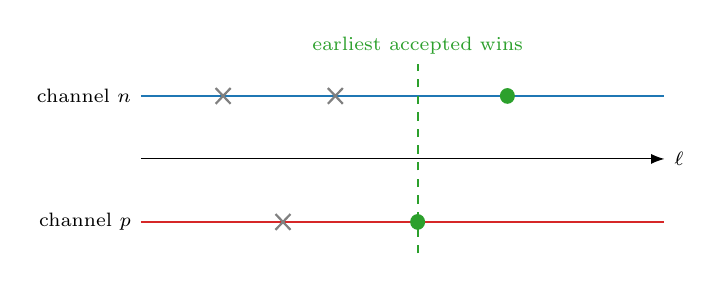
\begin{tikzpicture}[x=0.95cm]
  \draw[-{Latex}] (0,0) -- (7,0) node[right,font=\scriptsize]{$\ell$};
  \node[font=\scriptsize,anchor=east] at (0,0.8) {channel $n$};
  \node[font=\scriptsize,anchor=east] at (0,-0.8) {channel $p$};
  \draw[aBlue,thick] (0,0.8) -- (7,0.8); \draw[bRed,thick] (0,-0.8) -- (7,-0.8);
  \foreach \x in {1.1,2.6} \draw[gray,thick] (\x-0.1,0.7)--(\x+0.1,0.9) (\x-0.1,0.9)--(\x+0.1,0.7);
  \fill[okGreen] (4.9,0.8) circle(0.1);
  \foreach \x in {1.9} \draw[gray,thick] (\x-0.1,-0.9)--(\x+0.1,-0.7) (\x-0.1,-0.7)--(\x+0.1,-0.9);
  \fill[okGreen] (3.7,-0.8) circle(0.1);
  \draw[dashed,okGreen,thick] (3.7,-1.2) -- (3.7,1.2) node[above,font=\scriptsize]{earliest accepted wins};
\end{tikzpicture}
\column{0.48\textwidth}
\begin{derivbox}[Why this is right]
Each channel $c$ runs its own veto stream, so its first accepted point has density $\G_c(\ell)e^{-\int\G_c}$. The channels are independent, so channel $c$ wins at $\ell$ with density
\[
\G_c(\ell)\,e^{-\int\G_c}\prod_{c'\ne c}e^{-\int\G_{c'}}=\G_c(\ell)\,e^{-\int\sum_{c'}\G_{c'}} .
\]
Same as "total rate, then pick channel with $\G_c/\G$". \tagder
\end{derivbox}
\end{columns}
\vspace{4pt}
In (b) the channels are the target isospin, and \textbf{all candidates of all particles} are ordered in global time.
\end{frame}

\begin{frame}{The random target: draw it fresh at the candidate}
\small
\begin{derivbox}[Accept with $\G(T)/\Gh$ using a target $T\sim f$ drawn at the candidate]
\begin{columns}[T]
\column{0.5\textwidth}
Acceptance probability at a candidate:
\[
\int f(T)\,\frac{\G(T)}{\Gh}\,dT=\frac{\langle\G\rangle_T}{\Gh}
\]
so the thinned rate is $\langle\G\rangle_T$: \textbf{the average, automatically}.
\column{0.47\textwidth}
Law of the target, given acceptance:
\[
\frac{f(T)\,\G(T)}{\langle\G\rangle_T}
\]
exactly (a)'s $\Delta\to0$ target law.
\end{columns}
\end{derivbox}
\begin{keybox}
No Jensen error: the veto never needs $\langle\G\rangle_T$ explicitly. The only requirement is $\Gh\ge\G(T)$ for \emph{every} target $T$, at every point of the segment.
\end{keybox}
\begin{warnbox}[One exception, found by testing]
In NuWro's QE-SF ("consistent target") path, \code{make\_interaction} \emph{re-draws} target and isospin at the collision point; (b) keeps that. My first version reused the accepted target: 3\% too many collisions (6--10$\sigma$).
\end{warnbox}
\end{frame}

\begin{frame}{Building the bound $\Gh_c$: bound every factor}
\begin{tcolorbox}[colback=bRed!4,colframe=bRed,boxrule=0.8pt]
\[
\Gh_c=\underbrace{\bar\rho_{\max}\tfrac{N_c}{A}}_{\ge\rho_c}\;
\underbrace{\max_{E\in[E^{\rm eff}_{\min},E^{\rm eff}_{\max}]}\sigma_{\rm free}(E)}_{\text{exact: table knots}}\;
\underbrace{\frac{1}{1-a(\rho_{\max})/4}}_{\ge\text{medium factor}}\;
0.9^{[E_k^{\max}<40,\,np]}\;
\underbrace{\frac{\max_s\mathrm{corr}_c}{\min_r\mathrm{norm}_c}}_{\text{exact: knots}}\;\frac{1}{s_{\rm mfp}}
\]
\end{tcolorbox}
\small
\begin{columns}[T]
\column{0.5\textwidth}
\begin{itemize}
\item \textbf{Segment}: radial range $[r_{\rm lo},r_{\rm hi}]$ includes the closest approach; $s\in[s_0+\ell_a,s_0+\ell_b]$.
\item \textbf{Density}: max over a 4000-cell radial grid, plus a curvature allowance.
\item \textbf{Targets}: $|\mathbf T|\le k_F(\bar\rho_{\max}\max(Z_r,N_r)/A)$ gives the $\Ekeff$ range (slide ``Ingredient 2'').
\end{itemize}
\column{0.47\textwidth}
\begin{itemize}
\item \textbf{Tables are piecewise linear}: their maximum over an interval is at a knot or an end point, so these bounds are exact, not estimates.
\item \textbf{Pions}: the Oset tables are bilinear in $(E,\rho)$; max over $\rho$ at density knots.
\item \textbf{Every violation is counted.}
\end{itemize}
\end{columns}
\end{frame}

\begin{frame}{The one non-trivial bound: Pandharipande--Pieper}
\small
\begin{columns}[T]
\column{0.46\textwidth}
\begin{derivbox}[Claim: $\mathrm{mod}\le 1/(1-a/4)$]
Write $\mathbf F(\mathbf k)=\mathbf k/m^*(k)=\nabla\Phi(\mathbf k)$, $\Phi$ radial. Hessian eigenvalues:\\
tangential $1/m^*\ge1/M$;\\
radial $\varphi'(k)=\frac{1}{M}\Big[1+a\frac{1-3x}{(1+x)^3}\Big]$, $x=k^2/\lambda^2$.\\
$\min_x\frac{1-3x}{(1+x)^3}=-\frac14$ at $x=1$ $\Rightarrow\varphi'\ge\frac{1-a/4}{M}$.\\[2pt]
Strong convexity: $|\mathbf F(\mathbf k_1)-\mathbf F(\mathbf k_2)|\ge\frac{1-a/4}{M}|\mathbf k_1-\mathbf k_2|$.\\
With $m_3^*\le M$:
\[
\mathrm{mod}=\frac{|\Delta\mathbf k|/M}{|\Delta\mathbf F|}\frac{m_3^*}{M}\le\frac{1}{1-a/4}.\quad\text{\tagder}
\]
\end{derivbox}
\column{0.52\textwidth}
\centering
\includegraphics[height=0.72\textheight]{figs/pp_bound.pdf}\\
{\scriptsize Bound 1.20 at $\rho_0$; true maximum 1.06. \tagrun}
\end{columns}
\end{frame}

\begin{frame}{What $\G$ and $\Gh$ look like along a real chord}
\centering
\includegraphics[width=0.85\textwidth]{figs/chord.pdf}
\begin{columns}[T]
\column{0.55\textwidth}\small
Most of the gap between red and blue comes from bounding over the Fermi sea (sup of $\sigma$ over targets) and the density maximum on a 2 fm segment. The medium bound adds $\le$20\%.
\column{0.42\textwidth}
\begin{keybox}
Gap = rejected candidates = CPU time. It never changes the answer.
\end{keybox}
\end{columns}
\end{frame}

\begin{frame}{The price of bounding over the Fermi sea}
\begin{columns}[c]
\column{0.55\textwidth}
\includegraphics[width=\textwidth]{figs/eff.pdf}
\column{0.43\textwidth}
\begin{itemize}\small
\item Acceptance is limited by $\langle\sigma\rangle_T/\sup_T\sigma$.
\item For slow nucleons a co-moving target makes $\sup\sigma\sim13$ b against $\langle\sigma\rangle\sim$300 mb.
\item Measured acceptance in (b): \textbf{1--3\%}, 24--100 candidates per event. \tagrun
\end{itemize}
\begin{keybox}[Known fix, not implemented]
Draw the target as part of the proposal (importance-sample $T$). Estimated gain $\times3$--$30$ for slow nucleons.
\end{keybox}
\end{columns}
\end{frame}

\begin{frame}{Many particles: time order and re-anchoring}
\centering\small
\resizebox{0.92\textwidth}{!}{%
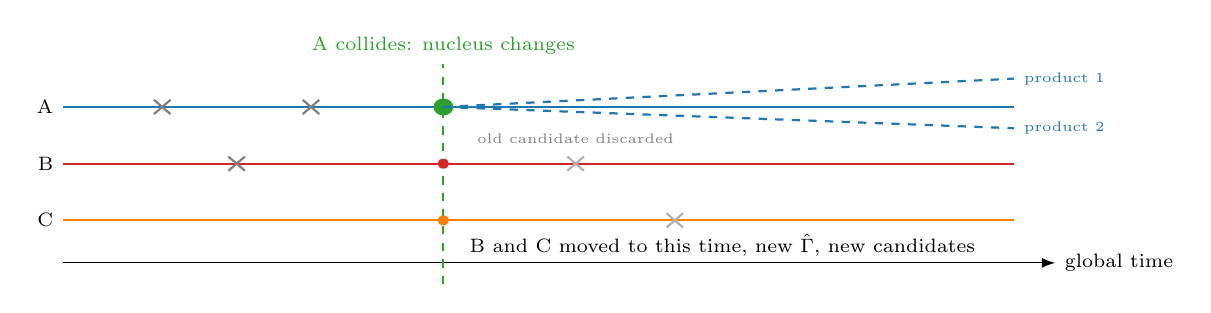
\begin{tikzpicture}[x=1.05cm,y=0.9cm]
  \draw[-{Latex}] (0,0) -- (12,0) node[right,font=\scriptsize]{global time};
  \foreach \y/\n/\c in {2.2/A/aBlue,1.4/B/bRed,0.6/C/orange} {\node[font=\scriptsize,anchor=east] at (0,\y) {\n}; \draw[\c,thick] (0,\y) -- (11.5,\y);}
  \foreach \x in {1.2,3.0} \draw[gray,thick] (\x-0.1,2.1)--(\x+0.1,2.3) (\x-0.1,2.3)--(\x+0.1,2.1);
  \fill[okGreen] (4.6,2.2) circle (0.12);
  \draw[dashed,okGreen,thick] (4.6,-0.3) -- (4.6,2.8) node[above,font=\scriptsize,align=center]{A collides: nucleus changes};
  \foreach \x in {2.1} \draw[gray,thick] (\x-0.1,1.3)--(\x+0.1,1.5) (\x-0.1,1.5)--(\x+0.1,1.3);
  \draw[gray!60,thick] (6.2-0.1,1.3)--(6.2+0.1,1.5) (6.2-0.1,1.5)--(6.2+0.1,1.3); \node[gray,font=\tiny] at (6.2,1.75) {old candidate discarded};
  \draw[gray!60,thick] (7.4-0.1,0.5)--(7.4+0.1,0.7) (7.4-0.1,0.7)--(7.4+0.1,0.5);
  \fill[bRed] (4.6,1.4) circle (0.07); \fill[orange] (4.6,0.6) circle (0.07);
  \node[font=\scriptsize,align=left,anchor=west] at (4.8,0.25) {B and C moved to this time, new $\Gh$, new candidates};
  \draw[aBlue,thick,dashed] (4.6,2.2) -- (11.5,2.6) node[right,font=\tiny]{product 1};
  \draw[aBlue,thick,dashed] (4.6,2.2) -- (11.5,1.9) node[right,font=\tiny]{product 2};
\end{tikzpicture}}
\vspace{2pt}
\begin{keybox}
Discarding pending candidates and redrawing is exact (memoryless). It is needed because a collision elsewhere can \emph{raise} another particle's rate, e.g.\ a jailed nucleon put back in.
\end{keybox}
\begin{warnbox}[Second thing found by testing]
1 violation in $1.9\times10^9$ candidates: a \emph{blocked} pion absorption had changed $Z_r,N_r$ (finding 2, Part 2) with no re-anchor. Fixed: such a change now triggers a re-anchor; 0 violations since. \tagrun
\end{warnbox}
\end{frame}

\begin{frame}{Leaving the nucleus is an event too}
\begin{columns}[T]
\column{0.5\textwidth}
Straight line $\mathbf r(\ell)=\mathbf r_0+\ell\,\hat{\mathbf d}$ meets the sphere $|\mathbf r|=R$ at
\begin{derivbox}[Ray--sphere crossing]
$|\mathbf r_0+\ell\hat{\mathbf d}|^2=R^2$
\[
\Rightarrow\ \ell_{\rm exit}=-\hat{\mathbf d}\!\cdot\!\mathbf r_0+\sqrt{(\hat{\mathbf d}\!\cdot\!\mathbf r_0)^2-r_0^2+R^2}
\]
\end{derivbox}
The last segment ends there. The exit competes with the channel candidates like a third ``channel'' whose time is known.
\column{0.47\textwidth}
\begin{itemize}
\item At the exit (b) calls the unmodified \code{leave\_nucleus()}: escape, or jail if $J\le w$.
\item Jailing in flight cannot happen ($J$ constant), but (b) checks it at every event anyway: \textbf{0 cases} in all runs. \tagrun
\item Energy thresholds (40 MeV, 280 MeV) are not events: $\G$ is evaluated exactly at each candidate, and the bound covers both sides.
\end{itemize}
\end{columns}
\end{frame}

\begin{frame}{The algorithm (b), complete}
\small
\begin{columns}[T]
\column{0.55\textwidth}
\small
\begin{tcolorbox}[colback=softGray,colframe=black!40,boxrule=0.5pt,left=3pt,right=3pt]
\textbf{for} each new particle: anchor at $(\mathbf r_0,t_0,s_0)$; for $c=n,p$: draw candidate from $\Gh_c$ on segment\\
\textbf{loop}:\\
\quad pick the particle/channel with the \textbf{earliest} event in global time\\
\quad move it straight there\\
\quad \textbf{if} exit: \code{leave\_nucleus}; if jailed $\to$ re-anchor all\\
\quad \textbf{else}: $X$ = \code{prepare\_interaction()} \ (fresh target)\\
\quad\quad accept if $u\,\Gh_c<\G_c$\\
\quad\quad \textbf{if} rejected: next candidate of $c$ from here\\
\quad\quad \textbf{if} accepted: \code{make\_interaction()}\\
\quad\quad\quad blocked $\to$ continue from here (re-anchor if nucleus changed)\\
\quad\quad\quad else \code{finalize\_interaction()}, re-anchor all others, add products
\end{tcolorbox}
\column{0.42\textwidth}
\begin{codebox}[In the patch (\code{kaskada7.cc})]
\code{sud\_cascade} \ 1563--1706\\
\code{sud\_bound} \ 1397--1505\\
candidate \code{:1527}, accept \code{:1640}\\
continue \code{:1653}, earliest \code{:1559, 1605--1612}
\end{codebox}
\begin{keybox}[Switch]
\code{-p kaskada\_sudakov=1}\\
\code{-p kaskada\_sudakov\_segment=2}\\
Off by default. With it off: bit-identical to (a).
\end{keybox}
\end{columns}
\end{frame}

% =====================================================================
\section{Part 5 -- Validation}

\begin{frame}{The five criteria}
\footnotesize
\begin{tabular}{p{3.0cm}p{5.2cm}p{5.2cm}}
\toprule
criterion & (a) NuWro & (b) patched\\
\midrule
1. $e^{-\int\G}$ not inverted in closed form & \textbf{No}: inverts $e^{-\G(\ell_0)\lambda}$ with $\G$ frozen (\code{:753, 768}); $\Delta$ is an accuracy knob & \textbf{Yes}: only $\Gh$ is inverted (\code{:1527})\\
2. Proposals from inverted $\Gh\ge\G$ & \textbf{No} majorant (\code{:747, 753}) & \textbf{Yes}: \code{sud\_bound}; violations counted\\
3. Accept with $\G/\Gh$ at candidate & \textbf{No}: only a Pauli veto (\code{:1001}) & \textbf{Yes}: fresh target, \code{u*gm<g} (\code{:1640})\\
4. Continue from rejected point, same channel & \textbf{No} rejection step & \textbf{Yes}: \code{sud\_draw(t,c,lb,...)} (\code{:1653})\\
5. Competing channels, earliest wins & \textbf{No}: total rate, then isospin (\code{:747, 754}) & \textbf{Yes}: two streams per particle, global time order\\
\bottomrule
\end{tabular}
\end{frame}

\begin{frame}{Test 1: a problem with a closed-form answer}
\begin{columns}[T]
\column{0.4\textwidth}
\small
Uniform sphere, constant (or random, mean-preserving) $\sigma$, absorb at the first collision. For an event with chord length $L$:
\[
P_{\rm int}=1-e^{-\rho\sigma L}
\]
\begin{derivbox}[KS test via probability-integral transform]
If depths $d$ follow the law, then
\[
u=\frac{1-e^{-\rho\sigma d}}{1-e^{-\rho\sigma L}}\sim U(0,1)
\]
for \emph{every} event, whatever its $L$. \tagder
\end{derivbox}
\column{0.56\textwidth}
\includegraphics[width=\textwidth]{figs/pit.pdf}
\scriptsize
\begin{tabular}{@{}p{4.3cm}cc@{}}
\toprule
& $P_{\rm int}-$exact & KS $p$\\
\midrule
(b): 9 runs, $L_{\rm seg}$ 0.3--20 fm, $\Gh\times1,\times3$, $\sigma$ 10--100 mb & $|z|\le1.2$ & 0.08--0.97\\
(a) 0.2 fm, constant $\sigma$ & $+0.8\sigma$ & 0.45\\
(a) 1 fm, random $\sigma$ & $-13\sigma$ & $10^{-12}$\\
\bottomrule
\end{tabular}\ \tagrun
\end{columns}
\end{frame}

\begin{frame}{Test 2: (b) reproduces (a) at $\Delta\to0$; it does not care about $L_{\rm seg}$}
\small
\begin{columns}[T]
\column{0.5\textwidth}
\textbf{(b) $-$ (a)$_{\Delta\to0}$} \tagrun
\begin{itemize}
\item $\sigma_R$ and $T$, 22 energies: $\chi^2=32/22$. The one $3.4\sigma$ point (T at 300 MeV) was rerun with $10^6$ events: (a, 0.05 fm) $0.6253\pm0.0005$, (b) $0.6253\pm0.0005$.
\item $\langle N_{\rm coll}\rangle$, 13 configurations: all within $\pm1.8\sigma$.
\item QE-SF branch: (a)$_0=2.110\pm0.003$, (b) $=2.116\pm0.003$.
\end{itemize}
\column{0.47\textwidth}
\textbf{Segment length $L_{\rm seg}=0.5,\,2,\,8$ fm} \tagrun
\begin{itemize}
\item $\sigma_R$, $T$ at 8 configurations: $\chi^2=21.9/16$.
\item $\langle N_{\rm coll}\rangle$: $\chi^2=20.4/16$.
\end{itemize}
\textbf{Regression} \tagrun
\begin{itemize}
\item NuWro has no automated physics tests at this commit (CI only builds).
\item Patched build with (b) off: \textbf{bit-identical} final states and counters to pristine NuWro, 4 configurations $\times$ 5000 events.
\item Patch on a fresh clone reproduces the development build bit for bit.
\end{itemize}
\end{columns}
\end{frame}

\begin{frame}{Test 3: data (both algorithms are equally off)}
\centering
\includegraphics[width=0.8\textwidth]{figs/res_data.pdf}\\
\small
\begin{tabular}{lccc}
\toprule
$\chi^2$ (data errors only) & $\sigma_R<100$ MeV (82 pts) & $\sigma_R\ge100$ MeV (17) & $T$ (15)\\
\midrule
(a), 0.2 fm & 6561 \ (model/data 0.75) & 548 \ (0.86) & 68.5 \ (0.90)\\
(b) & 6564 \ (0.75) & 550 \ (0.87) & 66.7 \ (0.90)\\
\bottomrule
\end{tabular}\ \tagrun\\[2pt]
{\scriptsize Data digitised from Isaacson et al.\ (2021); the 60.8/61.0 MeV pair is inconsistent. The disagreement is in the physics inputs, not the algorithm.}
\end{frame}

\begin{frame}{CPU per event}
\centering
\small
\begin{tabular}{lccccc}
\toprule
ms/event & (a) 0.2 & (a) 0.05 & (a) 0.025 & (b) & (b)/(a)$_{0.2}$\\
\midrule
$\sigma_R$, 30 MeV & 0.124 & 0.40 & 0.69 & 0.18 & 1.45\\
$\sigma_R$, 300 MeV & 0.133 & 0.40 & 0.73 & 0.12 & 0.90\\
$T$, 1 GeV & 0.20 & 0.62 & 1.16 & 0.33 & 1.70\\
QE-SF, 300 MeV & 0.21 & -- & 1.45 & 0.40 & 1.88\\
\bottomrule
\end{tabular}\ \tagrun\\[4pt]
{\scriptsize single core, idle machine, ROOT output included, startup subtracted}\\[8pt]
\begin{keybox}
Versus the \emph{default} (a): 0.9--1.9$\times$ the CPU. \quad Versus (a) at the step that removes the collision bias (0.025 fm): \textbf{3.5--6$\times$ faster}.
\end{keybox}
\end{frame}

% =====================================================================
\section{Part 6 -- Reweighting}

\begin{frame}{Event weights from the veto algorithm}
\footnotesize
\begin{columns}[T]
\column{0.52\textwidth}
Goal: reuse a sample made with $\G$ to describe $\G'=k\G$ (e.g.\ $k=s_{\rm mfp}/s'_{\rm mfp}$, or a cross-section scale).
\begin{derivbox}[Veto weights]
At every candidate, with the same $\Gh\ge\G'$:
\[
w\;\mathrel{*}=\;\begin{cases}\dfrac{\G'}{\G}=k & \text{accepted}\\[8pt] \dfrac{\Gh-\G'}{\Gh-\G} & \text{rejected}\end{cases}
\]
Check: the weighted accept probability is $\frac{\G}{\Gh}\cdot k=\frac{\G'}{\Gh}$, and the weighted reject probability is $\big(1-\frac{\G}{\Gh}\big)\frac{\Gh-\G'}{\Gh-\G}=1-\frac{\G'}{\Gh}$. So the weighted sample \emph{is} the veto algorithm for $\G'$. \tagder
\end{derivbox}
\column{0.45\textwidth}
\begin{derivbox}[(a) can do it too]
Likelihood ratio of each censored free path:
\[
w\;\mathrel{*}=\;\begin{cases}k\,e^{-(k-1)\G\lambda}&\lambda<\Delta\\ e^{-(k-1)\G\Delta}&\text{otherwise}\end{cases}
\]
This is exact for (a)'s own process, at its own step.
\end{derivbox}
\begin{derivbox}[Which is noisier?]
$\mathbb E W^2_{\rm veto}=\mathbb E\exp\!\int\frac{(\G'-\G)^2}{\G(1-\G/\Gh)}$\\
$\mathbb E W^2_{\rm exp}=\mathbb E\exp\!\int\frac{(\G'-\G)^2}{\G}$\\
The veto weights are always a bit noisier. \tagder
\end{derivbox}
\end{columns}
\end{frame}

\begin{frame}{Reweighting closes}
\centering
\includegraphics[width=0.8\textwidth]{figs/res_rw.pdf}
\begin{columns}[T]
\column{0.55\textwidth}\small
Reweighted to mfp 0.6/1.0 and NN scale 0.8/1.25 vs regenerated samples; 4 configurations $\times$ 5 observables. \tagrun\\
(a): $\chi^2=36.6/80$, max $|z|=1.7$. \ (b): $\chi^2=85.5/80$, max $|z|=2.6$; all $|z|>2$ in one configuration whose nominal sample is itself $+2.4\sigma$ high.
\column{0.42\textwidth}
\begin{keybox}
Reweighting works for both. (a) has slightly better ESS. So weights are \emph{not} something only (b) can give.
\end{keybox}
\end{columns}
\end{frame}

\begin{frame}{For comparison: how GENIE reweights FSI}
\begin{columns}[T]
\column{0.55\textwidth}
\small
Read in source (GENIE Reweight \texttt{5d45f8a}, Generator \texttt{e2e04f1}):
\begin{itemize}
\item Only the \textbf{hA} model is supported; any other FSI model is refused. \code{GReWeightINuke.cxx:83--90}
\item Only primary hadrons (status \code{kIStHadronInTheNucleus}) get weights. \code{:246}
\item Mean-free-path weight: $P'_{\rm surv}/P_{\rm surv}$ if it escaped, $(1-P')/(1-P)$ if it interacted. \code{GReWeightUtils.cxx:135--158}
\item $P_{\rm surv}$ is computed by \textbf{stepping} along the path. \code{INukeUtils2018.cxx:284--316}
\item Fate weights: rescale fate fractions.
\end{itemize}
\column{0.42\textwidth}
\begin{keybox}
GENIE: one-shot fate per primary hadron, survival probability by stepping, no hN cascade.\\[3pt]
NuWro (a) or (b): exact per-event weights for the \emph{whole} cascade, secondaries included.
\end{keybox}
\end{columns}
\end{frame}

% =====================================================================
\section{Part 7 -- Verdict}

\begin{frame}{Was it worth it?}
\begin{columns}[T]
\column{0.5\textwidth}
\textbf{What (b) gives}
\begin{itemize}\small
\item A genuine veto algorithm: all five criteria, exact for any bound, no step parameter.
\item Removes (a)'s 2--4\% undercount of secondary collisions, at 0.9--1.9$\times$ the CPU of default (a), 3.5--6$\times$ cheaper than shrinking the step.
\item Exact event weights with a step-free meaning.
\end{itemize}
\column{0.47\textwidth}
\textbf{Why I would not propose it as a replacement}
\begin{itemize}\small
\item What NuWro is tuned to ($\sigma_R$, $T$) has a step bias 10--50$\times$ below data errors and tuning.
\item The disagreement with data is in the inputs.
\item (a) is already exactly reweightable.
\item 655-line patch; every new physics factor needs a proven bound; 1--3\% acceptance until targets are sampled in the proposal.
\end{itemize}
\end{columns}
\vspace{4pt}
\begin{keybox}[Recommendation]
Send NuWro the four bugs and the step study. Offer (b) as an optional, off-by-default mode.
\end{keybox}
\end{frame}

\begin{frame}{What would change the recommendation}
\begin{enumerate}
\item \textbf{Observables that count secondary collisions.} Hadron multiplicities, calorimetric energy, neutron counting. A 2--4\% bias that depends on a numerical knob then becomes a real systematic.
\item \textbf{Systematic weights that should mean "physics only".} (a)'s weights reweight \emph{NuWro at 0.2 fm}; (b)'s reweight the continuous process itself.
\item \textbf{Prerequisite:} sample the target inside the proposal, so the acceptance stops being 1--3\% for slow nucleons.
\end{enumerate}
\vspace{6pt}
\begin{keybox}[Take-home]
The veto algorithm turns ``how small must my step be?'' into ``how tight is my bound?''. The first is an accuracy question, the second only a speed question. For NuWro today the accuracy question has a comfortable answer for $\sigma_R$ and $T$, and a percent-level one for collision counts.
\end{keybox}
\end{frame}

\appendix
\begin{frame}{Backup: where things live in NuWro (\texttt{f16c937})}
\small
\begin{tabular}{ll}
\toprule
what & where\\
\midrule
main loop, queue & \code{kaskada7.cc:72--93}, \code{kaskada7.h:54}\\
rate per step, free path & \code{kaskada7.cc:681--763} (\code{:747, 753})\\
move, jail check & \code{kaskada7.cc:766--819}\\
target nucleon, LFG & \code{nucleus.cc:101--164}, \code{nucleus.h:181--191}\\
NN cross sections, P\&P, 0.9 factor & \code{Interaction.cc:186--256, 326--391, 512--539}\\
process choice, orientation & \code{Interaction.cc:655--700}\\
pions & \code{Interaction.cc:403--424}, \code{Interaction.h:413--480}\\
Pauli & \code{kaskada7.cc:1001}, \code{nucleus.h:234--248}\\
SRC factor, mfp scale & \code{kaskada7.cc:720--745}, \code{data/input/kaskada\_NN\_corr\_1/6p6n.dat}\\
finalize, nucleus update & \code{kaskada7.cc:1027--1144}\\
beam placement & \code{nucleusmaker.h:17--46}\\
defaults (\code{step}=0.2, mfp 0.76) & \code{params\_all.h:135--136}\\
\bottomrule
\end{tabular}
\end{frame}

\end{document}
